% =====================================================================
%  CS426 - Mobile Development / Seminar Report
%  Topic: Clean Architecture (Android) - Case study: FieldFlow
%
%  Compile with:  pdflatex Report.tex   (run twice for the ToC)
%  No external assets required; all diagrams are TikZ.
% =====================================================================
\documentclass[11pt,a4paper]{article}

% ---------- Encoding & fonts ----------
\usepackage[T1]{fontenc}
\usepackage[utf8]{inputenc}
\usepackage{lmodern}
\usepackage{microtype}
\usepackage{amsmath}
\usepackage{amssymb}
% Allow long typewriter identifiers and file paths to break across lines.
\usepackage[htt]{hyphenat}
\setlength{\emergencystretch}{3em}

% ---------- Layout ----------
\usepackage[a4paper,margin=2.5cm]{geometry}
\usepackage{setspace}
\onehalfspacing
\usepackage{parskip}
\usepackage{fancyhdr}
\pagestyle{fancy}
\fancyhf{}
\fancyhead[L]{\small Clean Architecture on Android --- FieldFlow}
\fancyhead[R]{\small CS426 Seminar Report}
\fancyfoot[C]{\thepage}
\renewcommand{\headrulewidth}{0.4pt}

% ---------- Tables, graphics, misc ----------
\usepackage{booktabs}
\usepackage{tabularx}
\usepackage{longtable}
\usepackage{array}
\usepackage{multirow}
\usepackage{graphicx}
\usepackage{float}
\usepackage{enumitem}
\usepackage{xcolor}
\usepackage{caption}
\captionsetup{font=small,labelfont=bf}

% ---------- Diagrams ----------
\usepackage{tikz}
\usetikzlibrary{arrows.meta,positioning,shapes.geometric,fit,backgrounds,calc}

% ---------- Code listings ----------
\usepackage{listings}
\definecolor{codebg}{RGB}{248,248,248}
\definecolor{codekw}{RGB}{0,86,158}
\definecolor{codestr}{RGB}{27,124,60}
\definecolor{codecmt}{RGB}{120,120,120}
\definecolor{coderule}{RGB}{220,220,220}

\lstdefinelanguage{Kotlin}{
  keywords={package, as, typealias, this, super, val, var, fun, for, null, true,
    false, is, in, throw, return, break, continue, object, if, try, else, while,
    do, when, interface, class, data, sealed, internal, private, public,
    protected, override, abstract, suspend, operator, companion, import, by,
    open, out, reified, inline, const, lateinit, init, enum, annotation},
  keywordstyle=\color{codekw}\bfseries,
  ndkeywords={String, Int, Long, Boolean, List, Map, Flow, Unit, Set},
  ndkeywordstyle=\color{codekw},
  comment=[l]{//},
  morecomment=[s]{/*}{*/},
  commentstyle=\color{codecmt}\itshape,
  stringstyle=\color{codestr},
  morestring=[b]",
  sensitive=true,
}

\lstdefinestyle{ff}{
  backgroundcolor=\color{codebg},
  basicstyle=\ttfamily\scriptsize,
  breaklines=true,
  breakatwhitespace=true,
  captionpos=b,
  frame=single,
  rulecolor=\color{coderule},
  framesep=4pt,
  showstringspaces=false,
  numbers=none,
  tabsize=2,
  xleftmargin=2pt,
  columns=fullflexible,
  keepspaces=true,
}
\lstset{style=ff,language=Kotlin}

% ---------- Hyperlinks (load late) ----------
\usepackage[hidelinks]{hyperref}

% ---------- Helper macros ----------
\newcommand{\mdl}[1]{\texttt{#1}}
% \small is applied *outside* \texttt so that hyphenat's `htt' patch can still
% break long identifiers and paths at the end of a line.
\newcommand{\file}[1]{{\small\texttt{#1}}}

% =====================================================================
\begin{document}

% ---------------------------------------------------------------
% TITLE PAGE
% ---------------------------------------------------------------
\begin{titlepage}
\centering
\vspace*{1.5cm}

{\large\scshape University --- Faculty of Information Technology}\\[0.3cm]
{\large CS426 --- Mobile Development}\\[2.0cm]

\rule{\linewidth}{0.5pt}\\[0.5cm]
{\Huge\bfseries Clean Architecture on Android}\\[0.5cm]
{\LARGE A Case Study with FieldFlow}\\[0.4cm]
{\large\itshape Circuit-Based Feature-Modular Clean Architecture}\\[0.3cm]
\rule{\linewidth}{0.5pt}\\[2.0cm]

{\large\bfseries Seminar Report}\\[1.5cm]

% -----------------------------------------------------------
% TODO: replace with the real student IDs and names of the group.
% The ZIP file must be named:
%   <ID1>_<ID2>_<ID3>_<ID4>_CleanArchitecture.zip
% -----------------------------------------------------------
\begin{tabular}{ll}
\toprule
\textbf{Student ID} & \textbf{Full name / Role} \\
\midrule
\texttt{<StudentID1>} & Th\v{a}ng --- app shell, Circuit, navigation, inspection, integration \\
\texttt{<StudentID2>} & Huy --- domain models, business rules, use cases, domain tests \\
\texttt{<StudentID3>} & L\v{i}nh --- Room, data layer, repositories, offline-first, evidence \\
\texttt{<StudentID4>} & Linh --- dashboard, reports UI, design system, docs, demo \\
\bottomrule
\end{tabular}

\vfill
{\large Ho Chi Minh City, \today}
\end{titlepage}

% ---------------------------------------------------------------
\tableofcontents
\newpage

% ===============================================================
\section{Introduction}
% ===============================================================

\subsection{Problem}

Android applications tend to degrade in a characteristic way. Business rules
are written where they are first needed --- inside an \texttt{Activity}, a
composable, a \texttt{ViewModel}, or even inside a SQL query --- because that is
the shortest path to a working screen. Over time, three symptoms appear:

\begin{enumerate}[leftmargin=*]
  \item \textbf{Rules become untestable.} A validation rule that lives inside a
        composable cannot be verified without an emulator or a Robolectric
        runtime, so it is usually verified by hand, or not at all.
  \item \textbf{Rules become duplicated or lost.} When the same rule is needed
        on a second screen, it is copied. When storage changes, the copy in the
        DAO silently disappears.
  \item \textbf{Change becomes expensive.} Replacing a persistence library, a UI
        toolkit, or an export format touches code across the whole project
        because there is no boundary that says where infrastructure stops and
        policy begins.
\end{enumerate}

The underlying cause is not a lack of discipline but a lack of an
\emph{enforced} dependency direction. Naming conventions and package structure
express intent, but the compiler does not check them, so any file can import any
other file.

\subsection{Motivation}

Clean Architecture, as formulated by Robert C.\ Martin, proposes a single
organising principle --- the \emph{Dependency Rule} --- that source-code
dependencies must point inward, toward higher-level policy. Applied to Android,
this means that business rules must not know that Android, Jetpack Compose, or
Room exist.

The motivation for this seminar is to move that principle from a diagram to
something \emph{verifiable}. We therefore did not build a toy example. We built
and measured a real multi-module Android application, \textbf{FieldFlow}, in
which the architecture is enforced by the Gradle module graph rather than by
convention, and in which every claimed benefit is backed by a file, a build
script, or a passing test.

\subsection{Objectives}

\begin{enumerate}[leftmargin=*]
  \item Explain the Dependency Rule, dependency inversion, and the ports-and-%
        adapters pattern in the concrete vocabulary of an Android project.
  \item Show how Gradle modules convert an architectural convention into a
        \emph{compile-time} constraint.
  \item Demonstrate a complete end-to-end flow (UI $\rightarrow$ presenter
        $\rightarrow$ use case $\rightarrow$ port $\rightarrow$ adapter
        $\rightarrow$ Room) in working code.
  \item Show that business rules are testable on a plain JVM without any Android
        dependency.
  \item Show that infrastructure adapters are replaceable without touching the
        domain or the feature modules.
  \item Evaluate the approach honestly: measure its cost, state its limits, and
        say when a simpler architecture would be the better engineering choice.
\end{enumerate}

\subsection{Scope}

\textbf{In scope.} The architecture of the FieldFlow codebase as it exists in
the submitted source tree: 15 Gradle modules, a pure Kotlin/JVM domain layer, a
Room-backed data layer, eight Slack~Circuit feature modules, an application-level
composition root, and 187 automated unit tests (plus 4 instrumented tests run on
a Gradle-managed device in CI).

\textbf{Out of scope.} FieldFlow is a functional prototype and this report does
not claim otherwise. Authentication, a real backend, production cloud
synchronisation, push notifications, report scheduling and e-mail delivery, full
multi-section template authoring, and active/archive lifecycle controls are not
implemented. The pending-sync queue is drained at runtime, but by a deterministic
fake adapter standing in for a server that does not exist. Instrumented UI
coverage is four navigation and draft-persistence tests, so most screen-level
behaviour is still confirmed by hand. These exclusions are product-scope
decisions and do not affect the architectural claims, but they are stated so the
evaluation in Section~\ref{sec:eval} can be read fairly.

% ===============================================================
\section{Background}
% ===============================================================

\subsection{The Dependency Rule}

Clean Architecture organises a system as concentric circles. The inner circles
contain policy (what the software \emph{does}); the outer circles contain
mechanisms (how it talks to the world). The Dependency Rule states:

\begin{quote}\itshape
Source code dependencies must point only inward, toward higher-level policies.
Nothing in an inner circle can know anything at all about something in an outer
circle.
\end{quote}

Concretely: an inner-circle file must not contain an \texttt{import} of an
outer-circle package. The domain may not import Room; Room-facing code may
import the domain.

\subsection{Layers and their Android counterparts}

\begin{table}[H]
\centering
\small
\begin{tabularx}{\linewidth}{@{}l l X@{}}
\toprule
\textbf{Clean Architecture circle} & \textbf{FieldFlow module} & \textbf{Contents} \\
\midrule
Entities (enterprise rules)   & \mdl{:domain}          & \file{InspectionSession}, \file{InspectionTemplate}, \file{InspectionScore}, \file{MaintenanceIssue} \\
Use cases (application rules) & \mdl{:domain}          & \file{ValidateInspectionUseCase}, \file{CompleteInspectionUseCase}, \file{CalculateInspectionScoreUseCase} \\
Interface adapters            & \mdl{:feature:*}, \mdl{:data} & Circuit presenters and UI state; Room repository adapters and mappers \\
Frameworks \& drivers         & \mdl{:core:database}, \mdl{:app} & Room database, DAOs, migrations, Android \texttt{Context}, file storage \\
\bottomrule
\end{tabularx}
\caption{Mapping of Clean Architecture circles onto FieldFlow's Gradle modules.}
\end{table}

Entities and use cases share one module here. That is a deliberate
simplification: FieldFlow is a single application, so there is no second
application that would need to reuse the entities independently. The
\emph{boundary that matters} --- between policy and mechanism --- is still a hard
module boundary.

\subsection{Dependency inversion and ports/adapters}

The Dependency Rule appears to create a paradox: a use case must \emph{save}
data, but saving is an outer-circle concern. Dependency inversion resolves it.
The inner circle declares an interface expressing what it needs (a \emph{port});
the outer circle provides the implementation (an \emph{adapter}). The
source-code dependency now points inward even though control flow points
outward.

\begin{figure}[H]
\centering
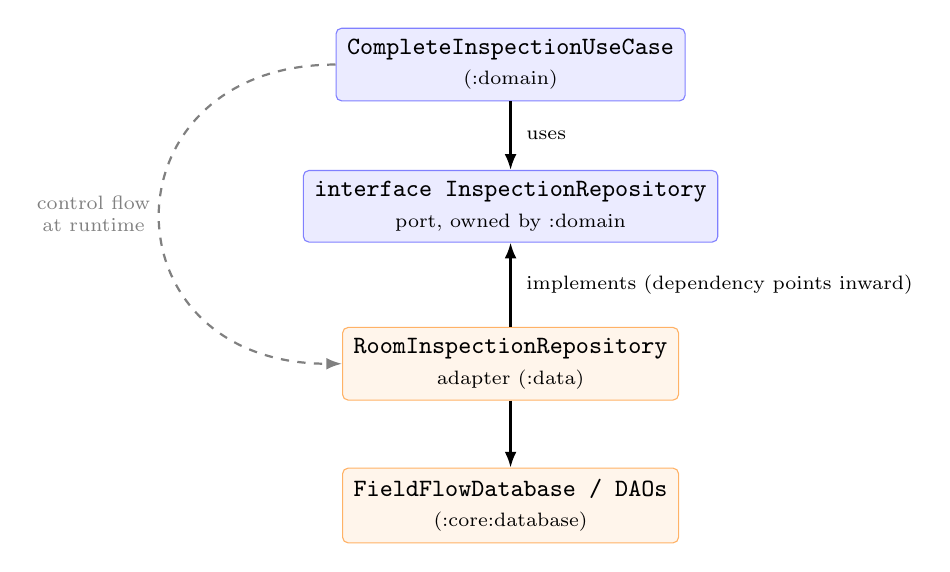
\begin{tikzpicture}[
  font=\small,
  box/.style={draw,rounded corners=2pt,minimum height=9mm,align=center,inner sep=4pt},
  inner/.style={box,fill=blue!8,draw=blue!50},
  outer/.style={box,fill=orange!8,draw=orange!60},
  dep/.style={-{Latex[length=2mm]},thick},
  ctrl/.style={-{Latex[length=2mm]},thick,dashed,gray}
]
\node[inner] (uc)   at (0,1.4) {\texttt{CompleteInspectionUseCase}\\\scriptsize(:domain)};
\node[inner] (port) at (0,-0.4) {\texttt{interface InspectionRepository}\\\scriptsize port, owned by :domain};
\node[outer] (imp)  at (0,-2.4) {\texttt{RoomInspectionRepository}\\\scriptsize adapter (:data)};
\node[outer] (db)   at (0,-4.2) {\texttt{FieldFlowDatabase / DAOs}\\\scriptsize(:core:database)};

\draw[dep] (uc) -- node[right=2pt,font=\scriptsize] {uses} (port);
\draw[dep] (imp) -- node[right=2pt,font=\scriptsize] {implements (dependency points inward)} (port);
\draw[dep] (imp) -- (db);
\draw[ctrl] (uc.west) .. controls (-5.2,1.4) and (-5.2,-2.4) .. node[left,font=\scriptsize,align=center] {control flow\\at runtime} (imp.west);
\end{tikzpicture}
\caption{Dependency inversion. The arrow from \mdl{:data} to \mdl{:domain} is a
compile-time dependency; the dashed arrow is runtime control flow. They point in
opposite directions, which is exactly the point.}
\end{figure}

\subsection{Slack Circuit as the presentation pattern}

FieldFlow structures its presentation layer with
\textbf{Slack~Circuit}~0.33.1, a Compose-native unidirectional data-flow
framework. Circuit defines four collaborating pieces:

\begin{center}
\texttt{Screen} $\rightarrow$ \texttt{Presenter} $\rightarrow$ immutable
\texttt{CircuitUiState} $\rightarrow$ \texttt{CircuitUiEvent} $\rightarrow$
Compose \texttt{Ui}
\end{center}

A \texttt{Screen} is a \texttt{Parcelable} navigation contract; a
\texttt{Presenter} is a \texttt{@Composable} function that observes flows and
emits immutable state; the \texttt{Ui} renders state and pushes events back
through an \texttt{eventSink}.

It is important to be precise about what Circuit is \emph{not}. Circuit is not a
replacement for Clean Architecture, and it is not "just MVVM with new names''.
Circuit organises the \emph{inside} of the outermost presentation circle. Clean
Architecture still decides which circle owns business policy. The two are
orthogonal, and this report treats them as such.

\subsection{Gradle modules as compile-time enforcement}

This is the mechanism that distinguishes an enforced architecture from a
documented one. In a single-module project, "the UI must not touch the
database'' is a rule a human must remember. In a multi-module project, the same
rule is expressed as an \emph{absence} in a build file:

\begin{lstlisting}[caption={\file{feature/inspection/build.gradle.kts} --- the
inspection feature can see the domain and shared UI, but \mdl{:data} and
\mdl{:core:database} are simply not on its compile classpath.}]
dependencies {
    implementation(platform(libs.androidx.compose.bom))
    implementation(project(":core:designsystem"))
    implementation(project(":core:navigation"))
    implementation(project(":domain"))
    // no ":data", no ":core:database" -- Room types cannot be imported here
    implementation(libs.androidx.compose.material3)
    implementation(libs.androidx.compose.runtime)
    implementation(libs.androidx.compose.ui)
    implementation(libs.circuit.retained)
    implementation(libs.circuit.runtime)
    implementation(libs.circuit.runtime.presenter)
    implementation(libs.circuit.runtime.ui)
    implementation(libs.kotlinx.coroutines.core)

    testImplementation(project(":core:testing"))
    testImplementation(libs.circuit.test)
    testImplementation(libs.junit)
    testImplementation(libs.kotlinx.coroutines.test)
}
\end{lstlisting}

An attempt to write \texttt{import com.topic11.cs426.data.RoomInspectionRepository}
inside \mdl{:feature:inspection} is a compilation error, not a code-review
comment. The architecture is checked by the build on every commit.

Domain purity is enforced by the same mechanism, one step more strictly:

\begin{lstlisting}[caption={\file{domain/build.gradle.kts} --- \mdl{:domain} is a
\texttt{java-library}, not an Android library. The Android SDK, Compose, Circuit
and Room are not available to it at all.}]
plugins {
    `java-library`
    alias(libs.plugins.kotlin.jvm)
}

dependencies {
    api(libs.kotlinx.coroutines.core)   // the only production dependency

    testImplementation(project(":core:testing"))
    testImplementation(libs.junit)
    testImplementation(libs.kotlinx.coroutines.test)
}
\end{lstlisting}

Note that \mdl{:domain} has exactly one production dependency:
\texttt{kotlinx-coroutines-core}. It is permitted because the repository ports
are reactive and return \texttt{Flow}; it introduces no framework coupling and
no Android coupling.

% ===============================================================
\section{Technical Approach}
% ===============================================================

\subsection{Architecture overview}

FieldFlow implements what we call \textbf{Circuit-Based Feature-Modular Clean
Architecture}: Clean Architecture supplies the dependency direction, feature
modularisation supplies ownership and compile-time isolation, Circuit structures
the presentation layer, and offline-first Room adapters supply persistence.

The application domain is facility and asset inspection. An inspector picks an
asset, selects an inspection template, answers checklist items (pass / fail /
not-applicable / measured value, with notes and evidence), saves drafts, reviews,
and completes the inspection. Completion triggers validation, weighted scoring,
automatic creation of maintenance issues for critical failures, and scheduling of
the next inspection. This is a genuine domain --- not CRUD --- which is what
makes it a fair subject for a Clean Architecture case study.

\begin{figure}[H]
\centering
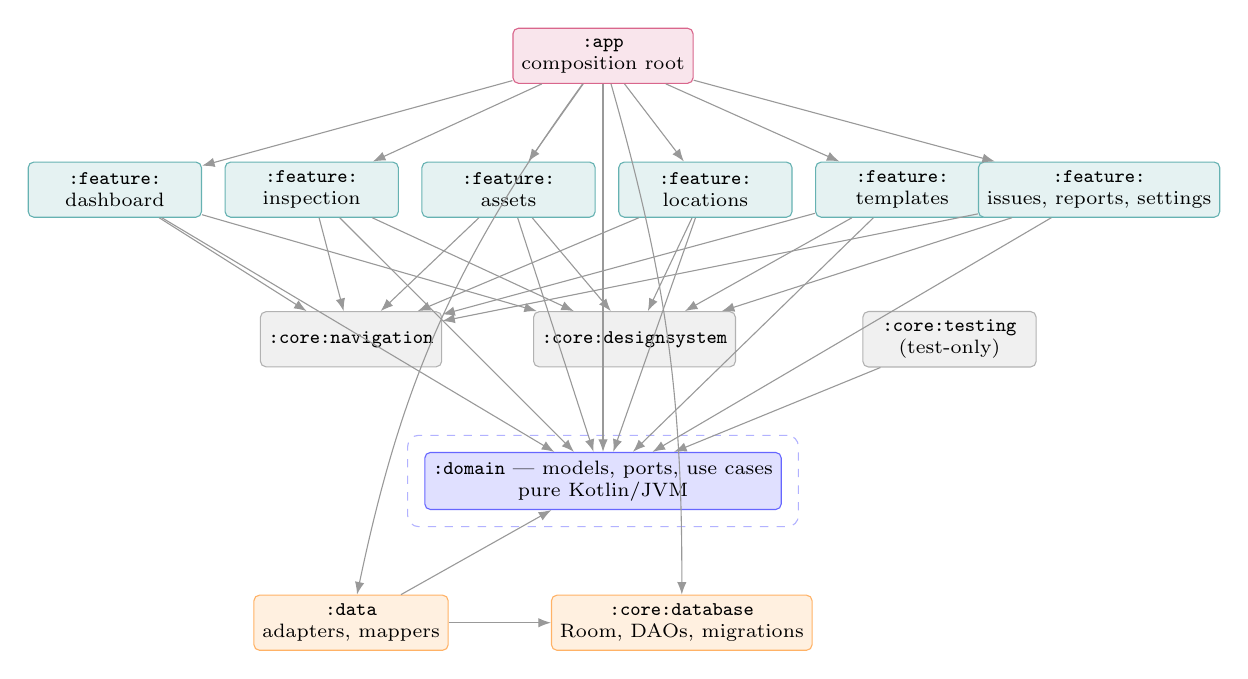
\begin{tikzpicture}[
  font=\scriptsize,
  m/.style={draw,rounded corners=2pt,minimum height=7mm,minimum width=22mm,align=center,inner sep=3pt},
  app/.style={m,fill=purple!10,draw=purple!60},
  feat/.style={m,fill=teal!10,draw=teal!60},
  core/.style={m,fill=gray!12,draw=gray!60},
  dom/.style={m,fill=blue!12,draw=blue!60,minimum width=34mm},
  dat/.style={m,fill=orange!12,draw=orange!60},
  a/.style={-{Latex[length=1.6mm]},gray!80}
]
% app
\node[app] (app) at (0,4.6) {\mdl{:app}\\composition root};

% features
\node[feat] (f1) at (-6.2,2.9) {\mdl{:feature:}\\dashboard};
\node[feat] (f2) at (-3.7,2.9) {\mdl{:feature:}\\inspection};
\node[feat] (f3) at (-1.2,2.9) {\mdl{:feature:}\\assets};
\node[feat] (f4) at ( 1.3,2.9) {\mdl{:feature:}\\locations};
\node[feat] (f5) at ( 3.8,2.9) {\mdl{:feature:}\\templates};
\node[feat] (f6) at ( 6.3,2.9) {\mdl{:feature:}\\issues, reports, settings};

% core
\node[core] (nav) at (-3.2,1.0) {\mdl{:core:navigation}};
\node[core] (ds)  at ( 0.4,1.0) {\mdl{:core:designsystem}};
\node[core] (tst) at ( 4.4,1.0) {\mdl{:core:testing}\\\scriptsize(test-only)};

% domain
\node[dom] (dom) at (0,-0.8) {\mdl{:domain} --- models, ports, use cases\\\scriptsize pure Kotlin/JVM};

% data
\node[dat] (dat) at (-3.2,-2.6) {\mdl{:data}\\adapters, mappers};
\node[dat] (db)  at ( 1.0,-2.6) {\mdl{:core:database}\\Room, DAOs, migrations};

\foreach \x in {f1,f2,f3,f4,f5,f6} \draw[a] (app) -- (\x);
\draw[a] (app) to[bend right=12] (dat);
\draw[a] (app) to[bend left=8]  (db);
\draw[a] (app.south) -- (dom.north);

\foreach \x in {f1,f2,f3,f4,f5,f6} {
  \draw[a] (\x) -- (nav);
  \draw[a] (\x) -- (ds);
  \draw[a] (\x) -- (dom);
}
\draw[a] (dat) -- (dom);
\draw[a] (dat) -- (db);
\draw[a] (tst) -- (dom);

\begin{scope}[on background layer]
\node[draw=blue!30,dashed,rounded corners,fit=(dom),inner sep=6pt] {};
\end{scope}
\end{tikzpicture}
\caption{The FieldFlow module graph (15 Gradle modules). Every arrow is a
compile-time dependency. \mdl{:domain} is the sink of the graph: many modules
depend on it, it depends on nothing in the project.}
\label{fig:modgraph}
\end{figure}

The essential shape of Figure~\ref{fig:modgraph} is:

\begin{center}
\texttt{Feature $\longrightarrow$ Domain $\longleftarrow$ Data}
\end{center}

Feature modules and the data layer both point at the domain. Neither can see the
other. \mdl{:app} sits above everything because it is the only module allowed to
know concrete implementations.

\subsection{Boundary rules}

The module graph is governed by rules that are documented in
\file{docs/architecture/MODULE\_GRAPH.md} and enforced by the build files:

\begin{table}[H]
\centering
\small
\begin{tabularx}{\linewidth}{@{}p{6.2cm} X@{}}
\toprule
\textbf{Allowed} & \textbf{Forbidden} \\
\midrule
\mdl{:app} may depend on everything.
& Feature modules must not depend on \mdl{:data} or \mdl{:core:database}. \\
\addlinespace
Features may depend on \mdl{:domain}, \mdl{:core:navigation}, \mdl{:core:designsystem}.
& Features must not import repositories, Room entities/DAOs, file adapters, sync adapters, or exporters. \\
\addlinespace
\mdl{:data} may depend on \mdl{:domain} and \mdl{:core:database}.
& \mdl{:domain} must not import Android, Compose, Circuit, Room, app, feature, or data packages. \\
\addlinespace
\mdl{:domain} may use Coroutines \texttt{Flow} (ports are reactive).
& Production source sets must not depend on \mdl{:core:testing}; only \mdl{:app} may assemble concrete adapters. \\
\bottomrule
\end{tabularx}
\caption{Boundary rules for the FieldFlow module graph.}
\end{table}

\subsection{The domain layer}

\mdl{:domain} contains 23 model files, 8 repository ports and 18 use-case files
(1{,}789 lines of production Kotlin). It has no Android code and can be compiled
and tested on a plain JVM.

\subsubsection{Business rules, and why they live here}

The rules FieldFlow owns are the reason the architecture pays for itself:

\begin{table}[H]
\centering
\small
\begin{tabularx}{\linewidth}{@{}p{5.4cm} X@{}}
\toprule
\textbf{Rule} & \textbf{Location} \\
\midrule
A required checklist item must be answered before completion & \file{ValidateInspectionUseCase.kt} \\
A critical item answered \texttt{Fail} must carry evidence & \file{ValidateInspectionUseCase.kt} \\
Score is weighted; \texttt{NotApplicable} is excluded from the denominator & \file{CalculateInspectionScoreUseCase.kt} \\
Only valid lifecycle transitions may complete an inspection & \file{CompleteInspectionUseCase.kt} \\
Every critical failure creates a maintenance issue & \file{CreateMaintenanceIssueUseCase.kt} \\
The next due date follows the template's, then the asset's, recurrence policy & \file{ScheduleNextInspectionUseCase.kt} \\
A report may only be generated from a completed inspection & \file{GenerateInspectionReportUseCase.kt} \\
\bottomrule
\end{tabularx}
\caption{Business rules implemented in \mdl{:domain}.}
\end{table}

Two of these rules, in their actual implementation:

\begin{lstlisting}[caption={\file{domain/.../usecase/ValidateInspectionUseCase.kt}
--- a pure function over two domain models. No repository, no coroutine, no
Android. This is the easiest kind of code to test and the hardest kind to break
accidentally.}]
class ValidateInspectionUseCase {

    operator fun invoke(
        session: InspectionSession,
        template: InspectionTemplate,
    ): ValidationResult {
        val errors = mutableListOf<InspectionValidationError>()
        val allItems = template.sections
            .flatMap { section -> section.items.map { it.id to it } }.toMap()
        val answerMap = session.answers.associateBy { it.checklistItemId }

        for ((itemId, item) in allItems) {
            val answer = answerMap[itemId]

            // RULE 1: Required item unanswered -> error
            if (item.required && (answer == null || answer.value == null)) {
                errors.add(InspectionValidationError.RequiredItemUnanswered(
                    itemId = itemId,
                    message = "Required item '${item.title}' has not been answered.",
                ))
            }

            // RULE 2: Critical + Fail must have evidence
            if (item.critical && answer?.value == ChecklistAnswerValue.Fail) {
                if (answer.evidenceIds.isEmpty()) {
                    errors.add(InspectionValidationError.CriticalFailureNeedsEvidence(
                        itemId = itemId,
                        message = "Critical item '${item.title}' requires evidence on failure.",
                    ))
                }
            }
        }
        return ValidationResult(isValid = errors.isEmpty(), errors = errors)
    }
}
\end{lstlisting}

\begin{lstlisting}[caption={\file{domain/.../usecase/CalculateInspectionScoreUseCase.kt}
--- weighted scoring with \texttt{NotApplicable} excluded from the denominator.
Expressing this in SQL inside a DAO would hide a business decision inside an
infrastructure detail.}]
for (section in template.sections) {
    for (item in section.items) {
        val answer = answerMap[item.id]

        // RULE 6: NotApplicable is excluded from the denominator
        if (answer?.value == ChecklistAnswerValue.NotApplicable) continue

        // RULE 5: Pass / Yes(true) earns weight, Fail / No(false) does not
        val scored = when (val value = answer?.value) {
            is ChecklistAnswerValue.Pass  -> true
            is ChecklistAnswerValue.YesNo -> value.value
            else -> false
        }
        totalWeight += item.weight
        if (scored) earnedWeight += item.weight
    }
}
\end{lstlisting}

\subsubsection{Ports}

The domain declares eight ports. Each expresses a business need, not a storage
technology:

\begin{table}[H]
\centering
\small
\begin{tabularx}{\linewidth}{@{}l X@{}}
\toprule
\textbf{Port} & \textbf{Business need it expresses} \\
\midrule
\file{InspectionRepository}          & observe summaries and one session, create, save draft, complete \\
\file{TemplateRepository}            & observe/load/save inspection templates \\
\file{AssetRepository}               & observe assets and locations, load and save them \\
\file{IssueRepository}               & observe/create/update maintenance issues \\
\file{ReportRepository}              & observe and persist export history \\
\file{ReportExporter}                & turn a report into an exported artefact \\
\file{EvidenceStore}                 & persist and delete evidence attached to answers \\
\file{AppearancePreferenceRepository}& observe and set the theme mode \\
\bottomrule
\end{tabularx}
\caption{Domain ports. Note that none of the names mention Room, files, JSON, PDF or Android.}
\end{table}

\begin{lstlisting}[caption={\file{domain/.../repository/InspectionRepository.kt}
--- the port. \texttt{Flow} is the only framework type it mentions.}]
interface InspectionRepository {
    fun observeInspectionSummaries(): Flow<List<InspectionSummary>>
    fun observeInspection(inspectionId: InspectionId): Flow<InspectionSession?>
    suspend fun getInspection(inspectionId: InspectionId): InspectionSession?
    suspend fun createInspection(
        assetId: String, assetName: String, templateId: String, startedAtMillis: Long,
    ): InspectionId
    suspend fun saveDraft(session: InspectionSession)
    suspend fun complete(completed: CompletedInspection)
}
\end{lstlisting}

\subsubsection{Orchestration}

\file{CompleteInspectionUseCase} is the clearest example of a use case as an
\emph{application} rule: it sequences other rules but contains no infrastructure.

\begin{lstlisting}[caption={\file{domain/.../usecase/CompleteInspectionUseCase.kt}
(abridged) --- all seven collaborators are domain types; none is a Room type.}]
class CompleteInspectionUseCase(
    private val inspectionRepository: InspectionRepository,
    private val templateRepository: TemplateRepository,
    private val assetRepository: AssetRepository,
    private val validateInspection: ValidateInspectionUseCase,
    private val calculateScore: CalculateInspectionScoreUseCase,
    private val createIssue: CreateMaintenanceIssueUseCase,
    private val scheduleNext: ScheduleNextInspectionUseCase,
) {
    suspend operator fun invoke(
        inspectionId: InspectionId,
        completedAtMillis: Long = System.currentTimeMillis(),
    ): CompleteInspectionResult {
        val session  = inspectionRepository.getInspection(inspectionId)
            ?: return CompleteInspectionResult.Error("Inspection not found")
        val template = templateRepository.getTemplate(session.templateId)
            ?: return CompleteInspectionResult.Error("Template not found")
        val asset    = assetRepository.getAsset(session.assetId)
            ?: return CompleteInspectionResult.Error("Asset not found")

        if (session.status != InspectionStatus.REVIEWING &&
            session.status != InspectionStatus.IN_PROGRESS) {
            return CompleteInspectionResult.ValidationFailed(listOf(
                InspectionValidationError.InvalidLifecycleTransition(
                    from = session.status, to = InspectionStatus.COMPLETED, /* ... */)))
        }

        val validation = validateInspection(session, template)
        if (!validation.isValid) return CompleteInspectionResult.ValidationFailed(validation.errors)

        val score      = calculateScore(session, template)
        val newIssues  = createIssue(findCriticalFailures(session, template), completedAtMillis)
        val nextDue    = scheduleNext(template, asset, completedAtMillis)

        inspectionRepository.complete(CompletedInspection(
            id = session.id, answers = session.answers, score = score, issues = newIssues,
            nextInspectionDueAtMillis = nextDue, completedAtMillis = completedAtMillis))

        return CompleteInspectionResult.Success(score, newIssues, nextDue, completedAtMillis)
    }
}
\end{lstlisting}

\subsection{The data layer}

\mdl{:core:database} owns the Room boundary: 11 entities, 5 DAOs, explicit
migrations, and \texttt{exportSchema = true} so schema JSON is versioned in git.

\begin{lstlisting}[caption={\file{core/database/.../FieldFlowDatabase.kt} (abridged).}]
@Database(
    entities = [
        LocationEntity::class, AssetEntity::class,
        InspectionTemplateEntity::class, InspectionSectionEntity::class,
        ChecklistItemEntity::class, InspectionEntity::class,
        InspectionAnswerEntity::class, EvidenceEntity::class,
        MaintenanceIssueEntity::class, ReportExportEntity::class,
        PendingSyncEntity::class,
    ],
    version = 3,
    exportSchema = true,
)
abstract class FieldFlowDatabase : RoomDatabase() {
    abstract fun catalogDao(): CatalogDao
    abstract fun inspectionDao(): InspectionDao
    abstract fun issueDao(): IssueDao
    abstract fun reportHistoryDao(): ReportHistoryDao
    abstract fun syncDao(): SyncDao
}
\end{lstlisting}

\mdl{:data} adapts that boundary to the domain ports. The canonical path is:

\begin{center}
Room entity $\rightarrow$ mapper $\rightarrow$ domain model $\rightarrow$
\texttt{Flow} $\rightarrow$ use case
\end{center}

A Room entity never escapes \mdl{:data}. The mapping is explicit, in five mapper
files, and this is a deliberate cost we accept in exchange for keeping storage
shape and business shape independent.

\begin{lstlisting}[caption={\file{data/.../RoomInspectionRepository.kt} (abridged)
--- the adapter composes DAO flows and maps records to domain models. The class
implements a domain interface, which is what makes the dependency point inward.}]
class RoomInspectionRepository(
    private val database: FieldFlowDatabase,
    private val inspectionIdFactory: () -> String = { "inspection-${UUID.randomUUID()}" },
) : InspectionRepository {

    private val inspectionDao = database.inspectionDao()

    override fun observeInspectionSummaries(): Flow<List<InspectionSummary>> =
        inspectionDao.observeInspectionSummaries()
            .map { records -> records.map { it.toDomain() } }
            .distinctUntilChanged()

    override fun observeInspection(inspectionId: InspectionId): Flow<InspectionSession?> =
        inspectionDao.observeInspectionSession(inspectionId.value)
            .flatMapLatest { record ->
                if (record == null) flowOf(null)
                else combine(
                    inspectionDao.observeAnswers(inspectionId.value),
                    inspectionDao.observeEvidence(inspectionId.value),
                ) { answers, evidence -> record.toDomain(answers, evidence) }
            }
            .distinctUntilChanged()
}
\end{lstlisting}

\mdl{:data} also supplies \file{AndroidEvidenceStore} (file-backed evidence),
\file{JsonReportExporter} and \file{PdfReportExporter} behind the single
\file{ReportExporter} port, \file{FieldFlowSampleDataSeeder}, and a deterministic
\file{FakeRemoteSyncAdapter}.

\subsection{The presentation layer}

Each feature module owns one slice of presentation and contains the same five
parts: a contract (state + events), a presenter, a Compose UI, Circuit
factories, and tests. Screen contracts themselves live in
\mdl{:core:navigation}, so features never import each other.

\begin{lstlisting}[caption={\file{feature/inspection/.../InspectionContracts.kt}
(abridged) --- the state machine is explicit and immutable.}]
@Immutable
sealed interface InspectionState : CircuitUiState {
    val eventSink: (InspectionEvent) -> Unit

    data class Loading(override val eventSink: (InspectionEvent) -> Unit) : InspectionState

    data class Editing(
        val title: String,
        val sections: List<InspectionSectionUi>,
        val currentSectionIndex: Int,
        val progress: InspectionProgress,
        val saveError: String? = null,
        override val eventSink: (InspectionEvent) -> Unit,
    ) : InspectionState

    data class Reviewing(/* ... */) : InspectionState
    data class ValidationFailed(
        val errors: List<ValidationError>, /* ... */) : InspectionState
    data class Completed(/* ... */) : InspectionState
}
\end{lstlisting}

The presenter is where the architecture is most visible, because of what is
\emph{absent} from its constructor:

\begin{lstlisting}[caption={\file{feature/inspection/.../InspectionPresenter.kt}
(abridged). Five collaborators, all of them domain use cases. There is no
repository, no DAO, no \texttt{Context}. The comment in the source --- ``Coordinates
the inspection workflow without owning business rules'' --- is enforced by the
module graph, not just asserted.}]
/** Coordinates the inspection workflow without owning business rules. */
internal class InspectionPresenter(
    private val screen: InspectionScreen,
    private val navigator: Navigator,
    private val observeInspection: ObserveInspectionUseCase,
    private val observeTemplate: ObserveTemplateUseCase,
    private val saveInspectionDraft: SaveInspectionDraftUseCase,
    private val validateInspection: ValidateInspectionUseCase,
    private val completeInspection: CompleteInspectionUseCase,
) : Presenter<InspectionState> {

    @Composable
    override fun present(): InspectionState {
        val sessionWithTemplate by remember(screen.inspectionId) {
            observeInspection(InspectionId(screen.inspectionId))
                .flatMapLatest { session ->
                    if (session == null) flowOf(null to null)
                    else observeTemplate(session.templateId).map { session to it }
                }
        }.collectAsState(initial = null to null)
        // ... maps domain session + template onto immutable UI state
    }
}
\end{lstlisting}

\subsection{The composition root}

\file{FieldFlowCompositionRoot.kt}, in \mdl{:app}, is the only place in the
codebase that knows concrete implementations. It opens Room with migrations,
constructs the adapters, injects them into domain use cases, registers Circuit
factories, schedules sample-data seeding on an app-scoped IO coroutine so that
\texttt{onCreate} is never blocked by database work, and starts the pending-sync
drain on that same scope.

The graph is owned by \file{FieldFlowApplication}, not by \file{MainActivity}: it
holds the Room handle and an application-scoped \texttt{CoroutineScope}, so it
must outlive Activity recreation. Creating it in the \texttt{Application} means a
configuration change no longer closes and reopens the database or cancels an
in-flight draft save.

\begin{lstlisting}[caption={\file{FieldFlowCompositionRoot.kt} (abridged) --- the
single point at which "which adapter?'' is answered.}]
fun create(applicationContext: Context): FieldFlowCompositionRoot {
    val database = Room.databaseBuilder(
        applicationContext, FieldFlowDatabase::class.java, FieldFlowDatabase.DATABASE_NAME,
    ).addMigrations(*FieldFlowMigrations.ALL).build()
    val appScope = CoroutineScope(SupervisorJob() + Dispatchers.IO)

    return try {
        val syncDao = database.syncDao()
        // No backend exists yet, so the adapter stands in for one.
        val remoteSyncAdapter = FakeRemoteSyncAdapter(
            syncDao = syncDao,
            scenario = AttemptBasedFakeSyncScenario(outcomesByAttempt = emptyMap()),
            clock = System::currentTimeMillis)

        createWithRepositories(
            database = database,
            appScope = appScope,
            inspectionRepository = RoomInspectionRepository(database),
            templateRepository   = RoomTemplateRepository(catalogDao),
            assetRepository      = RoomAssetRepository(catalogDao),
            issueRepository      = RoomIssueRepository(issueDao),
            reportRepository     = RoomReportRepository(database.reportHistoryDao()),
            reportExporter       = FieldFlowReportExporter(
                jsonReportExporter = JsonReportExporter(reportFileStorage),
                pdfReportExporter  = PdfReportExporter(reportFileStorage)),
            appearancePreferenceRepository =
                AndroidAppearancePreferenceRepository.create(applicationContext),
            evidenceStore        = AndroidEvidenceStore(/* ... */),
            reportActionHandler  = AndroidReportActionHandler(/* ... */),
            seedSampleData       = { FieldFlowSampleDataSeeder(database).seedIfEmpty() },
            pendingSyncDrain     = PendingSyncDrain(
                retryableCommands = syncDao.observeRetryableCommands(),
                sync = remoteSyncAdapter::sync),
        )
    } catch (throwable: Throwable) {
        // A half-built graph would leak the scope and the open database handle.
        appScope.cancel(); database.close(); throw throwable
    }
}

// ... later, use cases are built from *ports*, never from concrete classes:
val completeInspection = CompleteInspectionUseCase(
    inspectionRepository = inspectionRepository,   // type: InspectionRepository
    templateRepository   = templateRepository,
    assetRepository      = assetRepository,
    validateInspection   = validateInspection,
    calculateScore       = CalculateInspectionScoreUseCase(),
    createIssue          = CreateMaintenanceIssueUseCase(),
    scheduleNext         = ScheduleNextInspectionUseCase(),
)
\end{lstlisting}

The private helper \texttt{createWithRepositories} takes \emph{port} types as
parameters. That signature is what makes the whole graph substitutable: the same
function can be called with different adapters, and nothing else in the project
changes.

\subsection{Offline-first}

Room is the local source of truth. Reads are \texttt{Flow}-based, so a write in
one screen propagates to every observer automatically. Drafts are persisted, so
an inspection survives process death. A \texttt{PendingSyncEntity} table records
work that a future backend would replay: completing an inspection enqueues a
\texttt{PENDING} command, and the inspection reports as
\texttt{InspectionStatus.SYNC\_PENDING} until that command settles.

That queue now has a consumer. \file{PendingSyncDrain} (in \mdl{:app}) collects
\texttt{SyncDao.observeRetryableCommands()} on the app scope and hands each
command to \file{FakeRemoteSyncAdapter}, with exponential backoff capped at
60~seconds and a bounded attempt count
(\texttt{DEFAULT\_MAX\_SYNC\_ATTEMPTS}~$=5$) after which a command is left
\texttt{FAILED} rather than retried forever. Two details are worth noting because
they are the kind of defect a diagram cannot show. Without the drain, nothing
ever consumed the queue --- every completed inspection stayed \texttt{PENDING},
so the Dashboard "Sync pending'' tile only counted up. And because a sync is two
writes (claim, then settle), the pair runs inside \texttt{NonCancellable}:
cancelling between them would park the command in \texttt{SYNCING}, a state
\texttt{observeRetryableCommands} never returns, stranding the inspection with
nothing left to retry it.

The adapter is still a fake --- there is no server --- but the \emph{path} is
live, and it is exercised end to end against a real Room database in
\file{PendingSyncDrainEndToEndTest.kt}. Offline-first is therefore an
\emph{architectural} property here: the domain never knows whether data came from
cache or network, because it only ever sees domain models arriving through a
port. Replacing the fake with a real client is a change in \mdl{:data} plus one
argument in the composition root.

% ===============================================================
\section{Demo and Case Study}
% ===============================================================

\subsection{The application}

FieldFlow runs as a Compose application with a Circuit navigation shell. The
implemented, Room-backed workflows are: Dashboard, Inspection, Assets,
Locations, Templates, Issues, Reports, and Settings.

\begin{table}[H]
\centering
\small
\begin{tabularx}{\linewidth}{@{}l X@{}}
\toprule
\textbf{Screen} & \textbf{Implemented behaviour} \\
\midrule
Dashboard  & overview metrics (total / in-progress / sync-pending / open issues), continue-inspection card, status filters, start-inspection sheet that picks an asset and template and creates the draft \\
Inspection & sections, pass/fail/NA/measured answers, notes, evidence capture, draft save (including on system back), review, validation, completion \\
Assets     & list, detail, add/edit, location association, validation, start-inspection handoff \\
Locations  & list, search, detail, add/edit, validation (deletion omitted to protect asset associations) \\
Templates  & list, detail with sections/items, add template with an initial checklist item, metadata editing that preserves the checklist aggregate \\
Issues     & list with filters, detail, domain-validated lifecycle transitions \\
Reports    & completed-inspection candidates, report detail, JSON and PDF export, persisted export history, open/share \\
Settings   & System / Light / Dark appearance, persisted and applied at the theme root \\
\bottomrule
\end{tabularx}
\caption{Implemented FieldFlow workflows.}
\end{table}

\subsection{End-to-end trace: completing an inspection}

This is the flow we demonstrate live, because it crosses every boundary in the
architecture exactly once.

\begin{figure}[H]
\centering
\resizebox{\linewidth}{!}{%
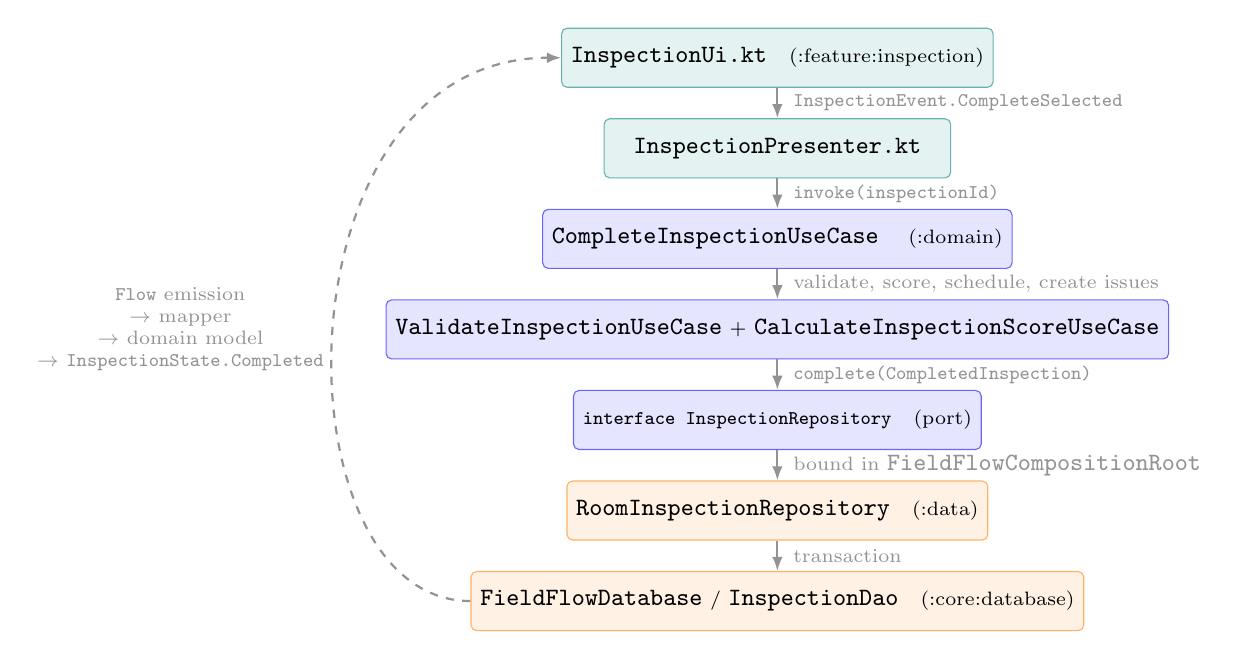
\begin{tikzpicture}[
  font=\scriptsize,
  n/.style={draw,rounded corners=2pt,minimum width=44mm,minimum height=7.5mm,align=center},
  ui/.style={n,fill=teal!10,draw=teal!60},
  dm/.style={n,fill=blue!10,draw=blue!60},
  dt/.style={n,fill=orange!10,draw=orange!60},
  a/.style={-{Latex[length=1.8mm]},thick,gray!85}
]
\node[ui] (n1) at (0,0)     {\file{InspectionUi.kt}\quad(:feature:inspection)};
\node[ui] (n2) at (0,-1.15) {\file{InspectionPresenter.kt}};
\node[dm] (n3) at (0,-2.30) {\file{CompleteInspectionUseCase} \quad(:domain)};
\node[dm] (n4) at (0,-3.45) {\file{ValidateInspectionUseCase} + \file{CalculateInspectionScoreUseCase}};
\node[dm] (n5) at (0,-4.60) {\texttt{interface InspectionRepository}\quad(port)};
\node[dt] (n6) at (0,-5.75) {\file{RoomInspectionRepository}\quad(:data)};
\node[dt] (n7) at (0,-6.90) {\file{FieldFlowDatabase} / \file{InspectionDao}\quad(:core:database)};

\draw[a] (n1) -- node[right=2pt] {\texttt{InspectionEvent.CompleteSelected}} (n2);
\draw[a] (n2) -- node[right=2pt] {\texttt{invoke(inspectionId)}} (n3);
\draw[a] (n3) -- node[right=2pt] {validate, score, schedule, create issues} (n4);
\draw[a] (n4) -- node[right=2pt] {\texttt{complete(CompletedInspection)}} (n5);
\draw[a] (n5) -- node[right=2pt] {bound in \file{FieldFlowCompositionRoot}} (n6);
\draw[a] (n6) -- node[right=2pt] {transaction} (n7);
\draw[a,dashed] (n7.west) .. controls (-6.4,-6.9) and (-6.4,0) ..
  node[left,align=center] {\texttt{Flow} emission\\$\rightarrow$ mapper\\$\rightarrow$ domain model\\$\rightarrow$ \texttt{InspectionState.Completed}} (n1.west);
\end{tikzpicture}}
\caption{The inspection completion flow. Each downward arrow crosses exactly one
architectural boundary; the dashed arrow is the reactive return path.}
\label{fig:e2e}
\end{figure}

Two observations make this the core of the demonstration:

\begin{itemize}[leftmargin=*]
  \item The presenter never decides whether the inspection is valid. It calls a
        use case and renders the result. Moving the validation rule requires
        editing one domain file, and no presentation file.
  \item Nothing above \file{InspectionRepository} in Figure~\ref{fig:e2e} knows
        that Room exists. Swapping persistence means editing
        \file{FieldFlowCompositionRoot.kt} and adding one class in \mdl{:data}.
\end{itemize}

\subsection{Verification method}

We verify the architecture at five levels rather than by inspection alone.

\begin{enumerate}[leftmargin=*]
  \item \textbf{Compile-time boundary checks.} The build itself is the primary
        test. If a feature module imported \mdl{:data}, compilation would fail.
        We verify the negative by reading the build files (no \texttt{:data}
        dependency in any \file{feature/*/build.gradle.kts}) and by the fact that
        the project compiles.
  \item \textbf{Pure JVM domain tests.} \mdl{:domain} tests run with
        \texttt{:domain:test} --- a plain \texttt{java-library} test task, with no
        emulator, no Robolectric, and no Android SDK. That this task exists at
        all is evidence of domain purity.
  \item \textbf{Adapter and database tests.} DAO behaviour, migrations, draft
        recovery, pending-sync state, mappers, exporters and seeding are tested
        in \mdl{:core:database} and \mdl{:data}.
  \item \textbf{Presenter tests.} Each feature's presenter is tested against
        fakes from \mdl{:core:testing} using \texttt{circuit-test}, verifying
        state transitions without rendering Compose.
  \item \textbf{Instrumented tests in CI.} Four navigation and
        draft-persistence tests run on a Gradle-managed device (Pixel~6,
        API~35, \texttt{aosp-atd}) declared in \file{app/build.gradle.kts}, so
        \texttt{:app:ciDeviceDebugAndroidTest} is the same command locally and
        on CI. GitHub Actions runs it on every push and pull request to
        \texttt{main}.
\end{enumerate}

The device is pinned to API~35 rather than 36, which would match
\texttt{targetSdk}, for two measured reasons: the ATD image only reaches the
stable SDK channel up to 35, and on the API~36 image the two
\texttt{Espresso.pressBack()} tests fail headless with
\texttt{RootViewWithoutFocusException} because the app window never takes focus.
The cost, stated plainly, is that behaviour specific to targeting API~36 goes
uncovered by CI.

Screen-level acceptance beyond those four tests is still performed by hand using
\file{docs/demo/FINAL\_MANUAL\_ACCEPTANCE\_CHECKLIST.md}.

The verification command used for the results below is:

\begin{lstlisting}[language={},caption={Module-scoped verification (PowerShell).}]
.\gradlew.bat :domain:test :data:testDebugUnitTest :core:database:testDebugUnitTest ^
  :app:testDebugUnitTest :feature:dashboard:testDebugUnitTest ^
  :feature:assets:testDebugUnitTest :feature:locations:testDebugUnitTest ^
  :feature:templates:testDebugUnitTest :feature:inspection:testDebugUnitTest ^
  :feature:issues:testDebugUnitTest :feature:reports:testDebugUnitTest ^
  :feature:settings:testDebugUnitTest --no-daemon
\end{lstlisting}

\subsection{Results}

\begin{table}[H]
\centering
\small
\begin{tabular}{@{}l r r r r@{}}
\toprule
\textbf{Module} & \textbf{Files} & \textbf{Prod.\ LOC} & \textbf{Test LOC} & \textbf{Tests} \\
\midrule
\mdl{:domain}              & 54  & 1{,}789 & 952   & 34 \\
\mdl{:data}                & 28  & 1{,}992 & 1{,}134 & 35 \\
\mdl{:core:database}       & 16  & 1{,}125 & 674   & 11 \\
\mdl{:core:navigation}     & 1   & 309     & --    & -- \\
\mdl{:core:designsystem}   & 7   & 531     & --    & -- \\
\mdl{:core:testing}        & 5   & 430     & --    & -- \\
\mdl{:app}                 & 14  & 957     & 600   & 16 \\
\mdl{:feature:dashboard}   & 11  & 1{,}987 & 570   & 20 \\
\mdl{:feature:inspection}  & 7   & 1{,}397 & 1{,}265 & 40 \\
\mdl{:feature:assets}      & 5   & 1{,}211 & 233   & 6  \\
\mdl{:feature:locations}   & 5   & 905     & 116   & 3  \\
\mdl{:feature:templates}   & 5   & 1{,}446 & 286   & 8  \\
\mdl{:feature:issues}      & 5   & 885     & 187   & 5  \\
\mdl{:feature:reports}     & 5   & 1{,}248 & 291   & 5  \\
\mdl{:feature:settings}    & 5   & 349     & 129   & 4  \\
\midrule
\textbf{Total} & \textbf{173} & \textbf{16{,}561} & \textbf{6{,}437} & \textbf{187} \\
\bottomrule
\end{tabular}
\caption{Measured size of the FieldFlow codebase. The \textbf{Files} column
counts production plus unit-test Kotlin files; \textbf{Test LOC} and
\textbf{Tests} cover unit tests only. The suite was executed with
\texttt{-{}-rerun-tasks} on 27~July~2026: 31 suites, 187 tests, 0 failures,
0 errors, 0 skipped, \texttt{BUILD SUCCESSFUL} in 3\,min~53\,s. Instrumented
code is counted separately: \file{FieldFlowNavigationSmokeTest.kt}, 223 lines,
4 tests, which are not part of the 187.}
\label{tab:metrics}
\end{table}

The numbers that matter architecturally are not the totals but their
\emph{distribution}:

\begin{itemize}[leftmargin=*]
  \item \textbf{Test-to-production ratio in \mdl{:domain} is 0.53} (952 test
        lines to 1{,}789 production lines), second only to
        \mdl{:feature:inspection} at 0.91. That density is only achievable
        because domain tests need no Android runtime.
  \item \textbf{34 of the 187 tests run on a bare JVM} through
        \texttt{:domain:test}. Every other module's unit tests are Android
        unit tests, and the ones that touch Room or files
        (\mdl{:data}, \mdl{:core:database}, \mdl{:app}) need Robolectric. If
        business rules lived in composables, those 34 tests would need it too.
  \item \textbf{\mdl{:domain} has one production dependency.} Its 1{,}789 lines
        are coupled to \texttt{kotlinx-coroutines-core} and nothing else.
  \item \textbf{Zero feature modules depend on \mdl{:data}.} This was verified
        across all eight \file{feature/*/build.gradle.kts} files.
\end{itemize}

Representative domain test names, taken directly from
\file{DomainBusinessRulesTest.kt}, show that the tests are written in the
language of the business rather than the language of the framework:

\begin{lstlisting}[caption={\file{domain/src/test/.../DomainBusinessRulesTest.kt}
--- test names as executable specification.}]
fun `cannotCompleteWithUnansweredRequiredItem`()
fun `criticalFailureRequiresEvidence`()
fun `criticalFailureCreatesIssue`()
fun `notApplicableIsExcludedFromScore`()
fun `invalidLifecycleTransitionIsRejected`()
fun `reportRequiresCompletedInspection`()
fun `nextInspectionDateUsesRecurrencePolicy`()
fun `nextInspectionDateFallsBackToAssetPolicyWhenTemplateHasNoPolicy`()
fun `critical issue IDs remain stable when completion is retried`()
\end{lstlisting}

\subsection{Case study: replacing an adapter}

The strongest practical claim of Clean Architecture is replaceability, so we
tested it rather than asserting it. FieldFlow ships more than one adapter behind
the same ports:

\begin{itemize}[leftmargin=*]
  \item the five \file{Room*Repository} adapters
        (\file{Inspection}, \file{Template}, \file{Asset}, \file{Issue},
        \file{Report}) --- the product runtime;
  \item \file{FakeInspectionRepository} (in \mdl{:data}) and the four fakes in
        \mdl{:core:testing} (\file{FakeAssetRepository},
        \file{FakeTemplateRepository}, \file{FakeIssueRepository},
        \file{RecordingInspectionRepository}) --- deterministic in-memory
        adapters used by presenter tests and adapter-swap experiments;
  \item two exporters, \file{JsonReportExporter} and \file{PdfReportExporter},
        behind the single \file{ReportExporter} port --- the clearest case,
        because both are production adapters and the domain distinguishes them
        only by a \file{ReportFormat} argument on \texttt{export}.
\end{itemize}

Switching the inspection adapter means passing a different argument to
\texttt{createWithRepositories}. The diff touches \mdl{:app} only. \mdl{:domain}
is unchanged; all eight feature modules are unchanged; every use case is
unchanged; and the presenter tests continue to pass because they were never
coupled to storage in the first place. This is dependency inversion producing a
concrete, measurable result rather than a diagram.

We should be precise about the limit of this claim. An earlier revision of the
project carried a parallel \file{DemoRepositories.kt} --- a complete second
adapter set for every port --- and that file has since been deleted, because once
the Room adapters worked it was dead weight that still had to compile. So what we
demonstrate today is one port swapped at a time against a fake, plus one port
(\file{ReportExporter}) with two live implementations. That is enough to show the
seam is real; it is not the same as running the whole application on a second
persistence stack, and we do not claim it is.

% ===============================================================
\section{Evaluation}
\label{sec:eval}
% ===============================================================

\subsection{Advantages observed}

\begin{table}[H]
\centering
\small
\begin{tabularx}{\linewidth}{@{}p{3.5cm} X@{}}
\toprule
\textbf{Benefit} & \textbf{Evidence in this codebase} \\
\midrule
Separation of concerns & Rules live in \file{ValidateInspectionUseCase.kt}; \file{InspectionUi.kt} only renders state. \\
Testability            & 34 domain tests run on a bare JVM via \texttt{:domain:test}, with no Android runtime; 187 unit tests pass in under 4 minutes. \\
Replaceability         & Room adapters and in-memory fakes satisfy the same ports, and JSON/PDF exporters share one port; switching touches \mdl{:app} only. \\
Compile-time safety    & No \file{feature/*/build.gradle.kts} declares \mdl{:data}; violations fail the build. \\
Framework isolation    & \mdl{:domain} has one production dependency and no Android, Compose, Circuit, or Room import. \\
Parallel development   & Four members owned \mdl{:app}/\mdl{:feature:inspection}, \mdl{:domain}, \mdl{:data}/\mdl{:core:database}, and dashboard/reports/design system, meeting only at domain contracts. \\
Scalability            & Adding \mdl{:feature:settings} required a new module, a screen contract, and two composition-root lines --- no change to existing features. \\
\bottomrule
\end{tabularx}
\caption{Benefits, each tied to something checkable in the source tree.}
\end{table}

The parallel-development benefit deserves emphasis because it is the one most
often claimed and least often examined. FieldFlow's four members agreed the
domain contracts first and then worked on role-scoped branches --- the git
history shows \texttt{feat/domain-business-rules},
\texttt{codex/data-room-foundation} and \texttt{feat/inspection-workflow} being
merged in dependency order (domain $\rightarrow$ data $\rightarrow$ features
$\rightarrow$ integration) rather than in completion order. The only shared file
set was \mdl{:domain}, so contract changes were the one thing that required
cross-role review. We should be candid that this was not frictionless: the
history also contains several explicit conflict-resolution commits, mostly
around integration points.

\subsection{Limitations and costs}

We do not claim the architecture is free. The measured and observed costs are:

\begin{itemize}[leftmargin=*]
  \item \textbf{Structural overhead.} 15 Gradle modules, 15 build scripts, and a
        version catalog to keep consistent. Configuration time and IDE indexing
        both grow with module count.
  \item \textbf{Mapping cost.} Five mapper files exist solely to translate Room
        records into domain models. This is duplicated shape --- an entity and a
        model that often look similar --- and it must be maintained in step.
  \item \textbf{Indirection.} Reading the completion flow requires opening a
        presenter, a use case, a port, an adapter, and a DAO. For a newcomer,
        "where does this actually happen?'' is a real and recurring question.
  \item \textbf{Composition-root growth.} \file{FieldFlowCompositionRoot.kt} is
        349 lines of manual wiring with no dependency-injection framework, and
        \texttt{createWithRepositories} now takes 13 parameters. It is explicit
        and testable, but it grows linearly with every feature and is the single
        most conflict-prone file in the repository.
  \item \textbf{Learning curve.} Circuit plus Clean Architecture plus
        multi-module Gradle is three unfamiliar things at once. The cost was paid
        during the first days of the project, not amortised over it.
  \item \textbf{Enforcement has gaps.} Gradle prevents feature $\rightarrow$ data
        imports, but nothing mechanically prevents a business rule from being
        written inside a presenter. That boundary is still maintained by review
        and by convention.
  \item \textbf{Verification is still unit-heavy.} 187 unit tests against 4
        instrumented tests. CI now runs the instrumented suite on a managed
        device on every push, which closed the worst of the gap --- but those
        four tests cover navigation and draft persistence only. Most
        screen-level behaviour across the eight features is still confirmed by
        hand, and the API~35 device means API~36-specific behaviour is
        uncovered.
  \item \textbf{The offline-first story is only half-proven.}
        \file{PendingSyncDrain} is wired and tested end to end, but against
        \file{FakeRemoteSyncAdapter}. Conflict resolution, partial failure from
        a real server, and authentication are the parts of synchronisation that
        are genuinely hard, and none of them has been attempted here.
\end{itemize}

\subsection{Trade-offs}

\begin{table}[H]
\centering
\small
\begin{tabularx}{\linewidth}{@{}p{3.6cm} X X@{}}
\toprule
\textbf{Trade-off} & \textbf{What we gained} & \textbf{What we paid} \\
\midrule
Modules vs.\ packages     & compile-time enforcement, clear ownership & build configuration, slower cold builds \\
Ports vs.\ direct calls   & replaceable storage, JVM-testable rules & one interface + one adapter per capability \\
Mappers vs.\ shared models& storage schema and business model evolve independently & duplicated shape, mapping code to maintain \\
Use cases vs.\ fat presenters & rules testable and reusable across screens & more small classes, more indirection \\
Manual DI vs.\ Hilt/Dagger& no annotation processing, explicit and debuggable graph & a large hand-written root that grows with the app \\
\bottomrule
\end{tabularx}
\caption{The principal trade-offs, stated in both directions.}
\end{table}

The manual-DI choice is worth expanding. Hilt would shrink
\file{FieldFlowCompositionRoot.kt} substantially and remove the conflict
hot-spot. We chose manual wiring because it makes the dependency graph readable
in one file --- valuable for a seminar whose subject \emph{is} the dependency
graph --- and because it adds no KSP round to the build. For a production app of
this size, Hilt would likely be the better choice.

\subsection{Alternatives considered}

\begin{table}[H]
\centering
\small
\begin{tabularx}{\linewidth}{@{}p{4.1cm} X X@{}}
\toprule
\textbf{Alternative} & \textbf{Why it is attractive} & \textbf{Why we did not choose it} \\
\midrule
Single-module MVVM, ViewModel calls repository directly
& fewest files; fastest to a running screen; idiomatic Android
& validation, scoring, evidence and lifecycle rules would sit in ViewModels, needing Robolectric to test and being copied across screens \\
\addlinespace
Layered packages in one module (\texttt{ui/}, \texttt{domain/}, \texttt{data/})
& expresses the same layering with no Gradle overhead
& the layering is unenforced; a single stray import silently violates it, and nothing fails \\
\addlinespace
MVI with a reducer, no use-case layer
& excellent state predictability; one obvious place per screen
& rules end up inside reducers, so they are per-screen rather than shared, and cross-screen rules such as report eligibility have no home \\
\addlinespace
Clean Architecture with Hilt instead of manual DI
& removes the hand-written composition root
& adds an annotation-processing round and hides the dependency graph the seminar needs to show; a reasonable choice in production \\
\bottomrule
\end{tabularx}
\caption{Alternatives, and the specific reason each was rejected \emph{for this project}.}
\end{table}

\subsection{Conditions for use}

Clean Architecture is not universally correct, and the honest conclusion of this
case study is a conditional one.

\textbf{Use it when} the application owns non-trivial business rules that outlive
any single screen; when storage or delivery mechanisms are expected to change;
when several people must work in parallel without stepping on each other; when
rules must be tested cheaply and repeatedly; or when the product is expected to
live for years.

\textbf{Do not use it when} the application is essentially a UI over a table with
no rules of its own; when it is a prototype whose main risk is not shipping at
all; when the team is one person on a short deadline; or when nobody on the team
has used the pattern before and the deadline leaves no room to learn it. In those
cases a single module with ViewModels and a repository is the better engineering
decision, and adopting Clean Architecture would be over-engineering.

FieldFlow sits clearly on the first side of that line: it has seven documented
business rules, offline-first persistence, replaceable export and evidence
adapters, four parallel owners, and an explicit list of future integrations. That
is why the cost is justified here --- and why we would not claim it is justified
everywhere.

% ===============================================================
\section{Conclusion}
% ===============================================================

\subsection{Key findings}

\begin{enumerate}[leftmargin=*]
  \item \textbf{The Dependency Rule becomes real only when a tool enforces it.}
        The single highest-value decision in this project was making
        \mdl{:domain} a \texttt{java-library} rather than an Android library.
        That one line in a build file makes an entire category of architectural
        violation impossible to compile.
  \item \textbf{Testability is a consequence of the boundary, not an extra
        effort.} We did not work to make the domain testable; it is testable
        because it has one dependency. 34 business-rule tests run in seconds on
        a plain JVM, inside a 187-test suite that completes in under 4 minutes.
  \item \textbf{Replaceability is measurable.} Room adapters and in-memory fakes
        satisfy the same ports, two exporters share one port, and switching
        between any of them changes exactly one module --- \mdl{:app}.
  \item \textbf{Circuit and Clean Architecture are orthogonal.} Circuit organises
        the presentation circle; Clean Architecture decides which circle owns
        policy. Conflating them --- treating presenters as a place for rules ---
        would have dissolved the boundary while leaving the diagram intact.
  \item \textbf{The cost is real and concentrated.} It appears as 15 build
        scripts, five mapper files, and a 349-line composition root. It is
        justified by this domain; it would not be justified by a simple CRUD app.
  \item \textbf{A port with no adapter running is not a feature.} The
        \texttt{pending\_sync} table, its DAO and \file{FakeRemoteSyncAdapter}
        all existed and were unit-tested while nothing consumed the queue, so
        every completed inspection sat on "Sync pending'' forever. Clean
        Architecture makes the seam easy to fill correctly; it does nothing to
        tell you the seam is empty. Only running the app did.
\end{enumerate}

\subsection{Lessons learned}

\begin{itemize}[leftmargin=*]
  \item \textbf{Agree the contracts before writing implementations.} Our team
        settled the IDs, models and repository ports on day one. Every later
        change went through the sequence domain $\rightarrow$ data $\rightarrow$
        presentation. Contract-first work, more than the module graph itself, is
        what made four people working in parallel viable.
  \item \textbf{Merge in dependency order, not completion order.} Domain first,
        then data, then features, then integration. Merging by who finished first
        produced conflicts; merging by dependency did not.
  \item \textbf{Boundaries a tool cannot check will erode.} The
        feature~$\nrightarrow$~data boundary held perfectly because Gradle
        enforces it. The "no business rules in presenters'' boundary required
        continuous review, because nothing enforces it.
  \item \textbf{Write the trade-offs down.} The most useful artefact for the
        seminar was not the diagram but the honest list of costs. An architecture
        presented without its price is not an argument.
  \item \textbf{Distinguish implemented from planned --- and re-check the list.}
        We maintained a list of what is wired at runtime versus what exists only
        as infrastructure. \file{FakeRemoteSyncAdapter} sat on the second list
        for most of the project and has since moved to the first, which is
        exactly why the list has to be re-derived from the code rather than
        remembered. Claiming more than the code does, or less, would have
        undermined everything else in this report.
\end{itemize}

% ===============================================================
\section{AI Usage Statement}
% ===============================================================

% -----------------------------------------------------------------
% TODO: to be written before submission.
% Should describe: which AI tools were used, for which tasks
% (e.g. drafting, refactoring suggestions, documentation), and how
% every AI output was verified (compilation, unit tests, code review,
% comparison against official documentation).
% -----------------------------------------------------------------

\textit{[To be completed before submission.]}

% ===============================================================
\begin{thebibliography}{99}
\addcontentsline{toc}{section}{References}

\bibitem{martin2017}
R.~C.~Martin, \emph{Clean Architecture: A Craftsman's Guide to Software
Structure and Design}. Boston, MA: Prentice Hall, 2017.

\bibitem{martinblog}
R.~C.~Martin, ``The Clean Architecture,'' \emph{The Clean Code Blog}, 2012.
[Online]. Available:
\url{https://blog.cleancoder.com/uncle-bob/2012/08/13/the-clean-architecture.html}

\bibitem{cockburn}
A.~Cockburn, ``Hexagonal Architecture (Ports and Adapters),'' 2005. [Online].
Available: \url{https://alistair.cockburn.us/hexagonal-architecture/}

\bibitem{androidarch}
Android Developers, ``Guide to app architecture.'' [Online]. Available:
\url{https://developer.android.com/topic/architecture}

\bibitem{androidmodular}
Android Developers, ``Guide to Android app modularization.'' [Online]. Available:
\url{https://developer.android.com/topic/modularization}

\bibitem{room}
Android Developers, ``Save data in a local database using Room.'' [Online].
Available: \url{https://developer.android.com/training/data-storage/room}

\bibitem{roommigrate}
Android Developers, ``Migrate your Room database.'' [Online]. Available:
\url{https://developer.android.com/training/data-storage/room/migrating-db-versions}

\bibitem{compose}
Android Developers, ``Jetpack Compose.'' [Online]. Available:
\url{https://developer.android.com/compose}

\bibitem{circuit}
Slack, ``Circuit --- A Compose-driven architecture for Kotlin and Android
applications.'' [Online]. Available: \url{https://slackhq.github.io/circuit/}

\bibitem{flow}
JetBrains, ``Asynchronous Flow --- Kotlin Coroutines documentation.'' [Online].
Available: \url{https://kotlinlang.org/docs/flow.html}

\bibitem{gradle}
Gradle, ``Structuring Projects with Gradle --- Multi-Project Builds.'' [Online].
Available: \url{https://docs.gradle.org/current/userguide/multi_project_builds.html}

\bibitem{nowinandroid}
Google, ``Now in Android --- a fully functional Android app built entirely with
Kotlin and Jetpack Compose,'' GitHub repository. [Online]. Available:
\url{https://github.com/android/nowinandroid}

\end{thebibliography}

% ===============================================================
\appendix
\section{Building and Running FieldFlow}
% ===============================================================

Full setup instructions are in \file{SourceCode/README.md}. In summary:

\textbf{Prerequisites.} JDK~21; Android SDK platform \texttt{android-36.1};
Gradle wrapper 9.4.1 (included). Toolchain versions: AGP 9.2.1, Kotlin 2.2.10,
KSP 2.3.10, Compose BOM 2026.02.01, Room 2.8.4, Circuit 0.33.1. Minimum
supported device: API~24.

\begin{lstlisting}[language={},caption={Build and verification commands (PowerShell).}]
# list the module graph
.\gradlew.bat projects --no-daemon

# run every unit test (187 tests, all passing)
.\gradlew.bat :domain:test :data:testDebugUnitTest :core:database:testDebugUnitTest ^
  :app:testDebugUnitTest :feature:dashboard:testDebugUnitTest ^
  :feature:assets:testDebugUnitTest :feature:locations:testDebugUnitTest ^
  :feature:templates:testDebugUnitTest :feature:inspection:testDebugUnitTest ^
  :feature:issues:testDebugUnitTest :feature:reports:testDebugUnitTest ^
  :feature:settings:testDebugUnitTest --no-daemon

# lint, test and assemble the debug APK (what CI's first job runs)
.\gradlew.bat lintDebug test assembleDebug :app:assembleDebugAndroidTest --no-daemon

# instrumented suite on the Gradle-managed device -- same command CI uses.
# Provisions a Pixel 6 / API 35 / aosp-atd emulator on first run.
.\gradlew.bat :app:ciDeviceDebugAndroidTest --no-daemon

# instrumented suite on an already-attached device or emulator
.\gradlew.bat connectedDebugAndroidTest --no-daemon
\end{lstlisting}

No account, API key, or external service is required: FieldFlow is offline-first
and seeds its own sample data on first launch.

\section{Key Files for the Demonstration}

\begin{table}[H]
\centering
\small
\begin{tabularx}{\linewidth}{@{}p{7.2cm} X@{}}
\toprule
\textbf{File} & \textbf{What it demonstrates} \\
\midrule
\file{domain/build.gradle.kts}                 & domain purity: a \texttt{java-library}, one dependency \\
\file{feature/inspection/build.gradle.kts}     & the absent \mdl{:data} dependency \\
\file{domain/.../ValidateInspectionUseCase.kt} & business rules as pure functions \\
\file{domain/.../InspectionRepository.kt}      & a port owned by the inner circle \\
\file{data/.../RoomInspectionRepository.kt}    & an adapter implementing that port \\
\file{app/.../FieldFlowCompositionRoot.kt}     & the single place that knows concrete types \\
\file{app/.../PendingSyncDrain.kt}             & an outer-circle mechanism the domain never sees \\
\file{feature/.../InspectionPresenter.kt}      & a presenter that owns no rules \\
\file{domain/.../DomainBusinessRulesTest.kt} & rules verified without Android \\
\bottomrule
\end{tabularx}
\caption{Files to open during the live demonstration, in order.}
\end{table}

\end{document}
